 \documentclass[a4paper,10pt]{article}
 \usepackage{tikz}
 \usepackage{fullpage}
 \usetikzlibrary{positioning,shadows,arrows,trees,shapes,fit}
 \begin{document}
 \begin{figure}
 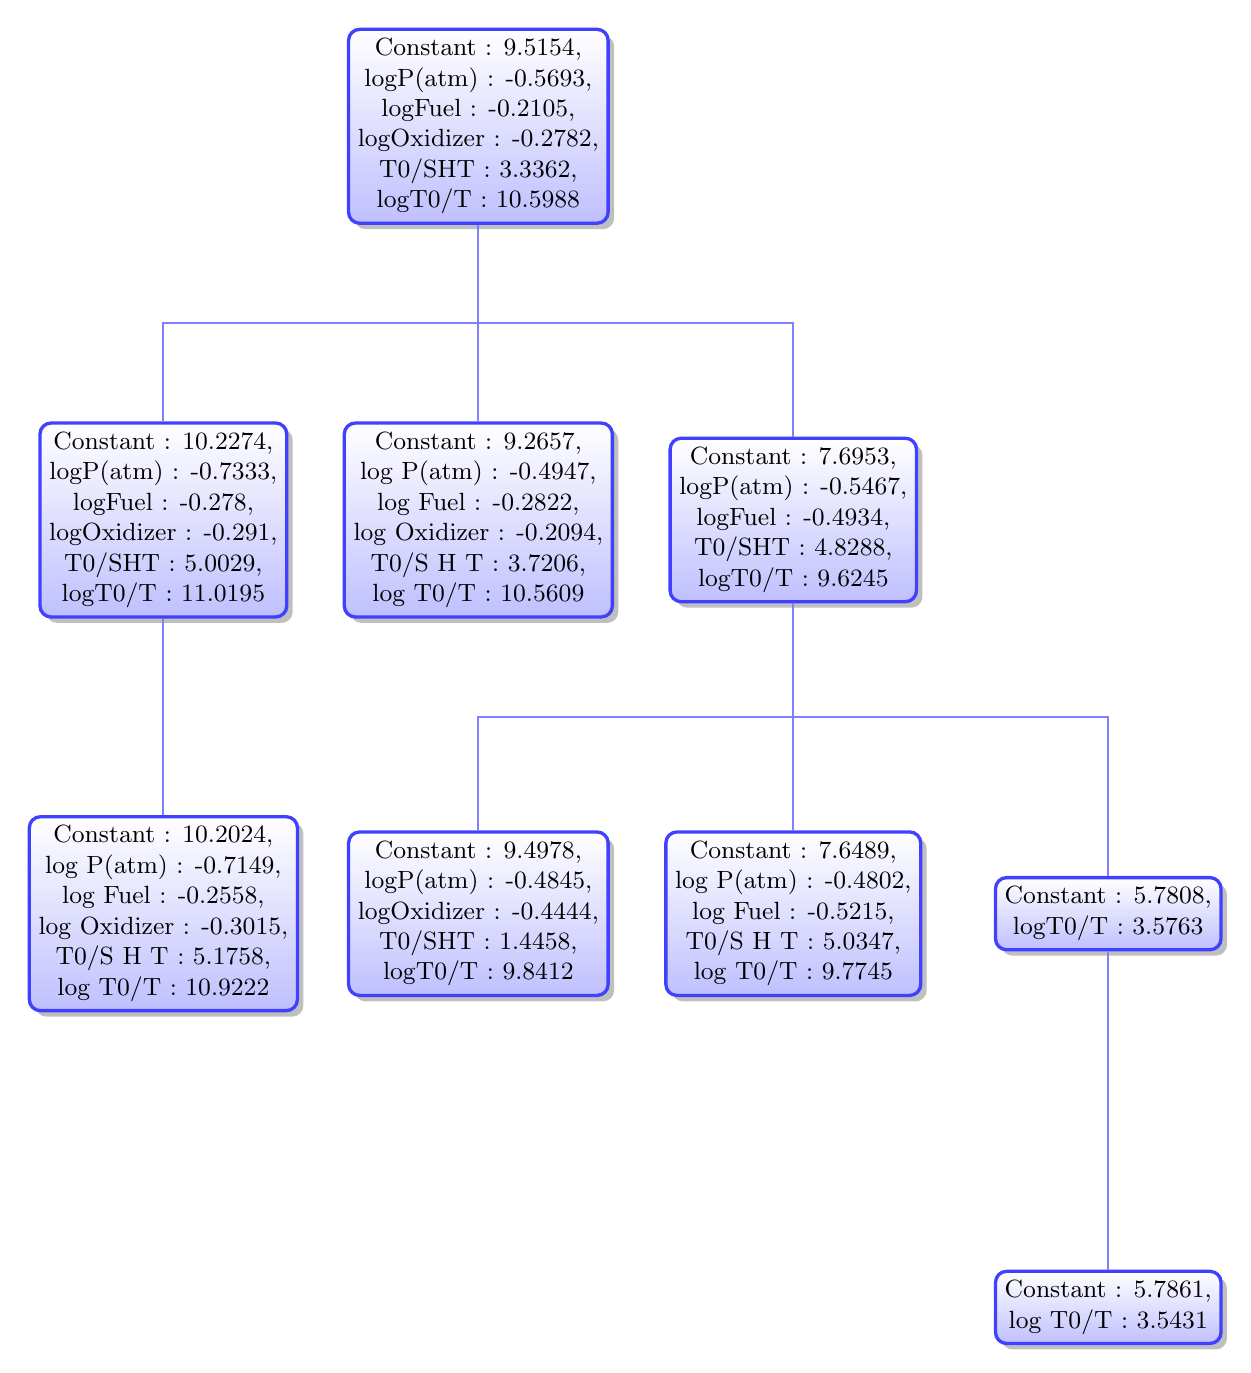
\begin{tikzpicture}
 [font=\small, edge from parent fork down, 
 every node/.style={top color=white, bottom color=blue!25, 
 	rectangle,rounded corners, minimum size=5mm, draw=blue!75,
	very thick, drop shadow, align=center},
 edge from parent/.style={draw=blue!50,thick},
 level 1/.style={sibling distance=4cm},
 level 2/.style={sibling distance=4cm}, 
 level 3/.style={sibling distance=4cm}, 
 level 4/.style={sibling distance=4cm}, 
 level 5/.style={sibling distance=4cm}, 
 level 6/.style={sibling distance=4cm}, 
 level distance=2cm,
 level distance=5cm,
 ]
\node { Constant : 9.5154,\\  logP(atm) : -0.5693,\\  logFuel : -0.2105,\\  logOxidizer : -0.2782,\\  T0/SHT : 3.3362,\\  logT0/T : 10.5988} %root
child { node { Constant : 10.2274,\\  logP(atm) : -0.7333,\\  logFuel : -0.278,\\  logOxidizer : -0.291,\\  T0/SHT : 5.0029,\\  logT0/T : 11.0195}  
child { node { Constant : 10.2024,\\  log P(atm) : -0.7149,\\  log Fuel  : -0.2558,\\  log Oxidizer  : -0.3015,\\  T0/S H  T : 5.1758,\\  log T0/T : 10.9222}  
 }
 }
child { node { Constant : 9.2657,\\  log P(atm) : -0.4947,\\  log Fuel  : -0.2822,\\  log Oxidizer  : -0.2094,\\  T0/S H  T : 3.7206,\\  log T0/T : 10.5609}  
 }
child { node { Constant : 7.6953,\\  logP(atm) : -0.5467,\\  logFuel : -0.4934,\\  T0/SHT : 4.8288,\\  logT0/T : 9.6245}  
child { node { Constant : 9.4978,\\  logP(atm) : -0.4845,\\  logOxidizer : -0.4444,\\  T0/SHT : 1.4458,\\  logT0/T : 9.8412}  
 }
child { node { Constant : 7.6489,\\  log P(atm) : -0.4802,\\  log Fuel  : -0.5215,\\  T0/S H  T : 5.0347,\\  log T0/T : 9.7745}  
 }
child { node { Constant : 5.7808,\\  logT0/T : 3.5763}  
child { node { Constant : 5.7861,\\  log T0/T : 3.5431} }
 }
 }
;\end{tikzpicture} 
 \caption{coefficient plot }  \end{figure}
\end{document} 
